\documentclass[1p]{elsarticle_modified}
%\bibliographystyle{elsarticle-num}

%\usepackage[colorlinks]{hyperref}
%\usepackage{abbrmath_seonhwa} %\Abb, \Ascr, \Acal ,\Abf, \Afrak
\usepackage{amsfonts}
\usepackage{amssymb}
\usepackage{amsmath}
\usepackage{amsthm}
\usepackage{scalefnt}
\usepackage{amsbsy}
\usepackage{kotex}
\usepackage{caption}
\usepackage{subfig}
\usepackage{color}
\usepackage{graphicx}
\usepackage{xcolor} %% white, black, red, green, blue, cyan, magenta, yellow
\usepackage{float}
\usepackage{setspace}
\usepackage{hyperref}

\usepackage{tikz}
\usetikzlibrary{arrows}

\usepackage{multirow}
\usepackage{array} % fixed length table
\usepackage{hhline}

%%%%%%%%%%%%%%%%%%%%%
\makeatletter
\renewcommand*\env@matrix[1][\arraystretch]{%
	\edef\arraystretch{#1}%
	\hskip -\arraycolsep
	\let\@ifnextchar\new@ifnextchar
	\array{*\c@MaxMatrixCols c}}
\makeatother %https://tex.stackexchange.com/questions/14071/how-can-i-increase-the-line-spacing-in-a-matrix
%%%%%%%%%%%%%%%

\usepackage[normalem]{ulem}

\newcommand{\msout}[1]{\ifmmode\text{\sout{\ensuremath{#1}}}\else\sout{#1}\fi}
%SOURCE: \msout is \stkout macro in https://tex.stackexchange.com/questions/20609/strikeout-in-math-mode

\newcommand{\cancel}[1]{
	\ifmmode
	{\color{red}\msout{#1}}
	\else
	{\color{red}\sout{#1}}
	\fi
}

\newcommand{\add}[1]{
	{\color{blue}\uwave{#1}}
}

\newcommand{\replace}[2]{
	\ifmmode
	{\color{red}\msout{#1}}{\color{blue}\uwave{#2}}
	\else
	{\color{red}\sout{#1}}{\color{blue}\uwave{#2}}
	\fi
}

\newcommand{\Sol}{\mathcal{S}} %segment
\newcommand{\D}{D} %diagram
\newcommand{\A}{\mathcal{A}} %arc


%%%%%%%%%%%%%%%%%%%%%%%%%%%%%5 test

\def\sl{\operatorname{\textup{SL}}(2,\Cbb)}
\def\psl{\operatorname{\textup{PSL}}(2,\Cbb)}
\def\quan{\mkern 1mu \triangleright \mkern 1mu}

\theoremstyle{definition}
\newtheorem{thm}{Theorem}[section]
\newtheorem{prop}[thm]{Proposition}
\newtheorem{lem}[thm]{Lemma}
\newtheorem{ques}[thm]{Question}
\newtheorem{cor}[thm]{Corollary}
\newtheorem{defn}[thm]{Definition}
\newtheorem{exam}[thm]{Example}
\newtheorem{rmk}[thm]{Remark}
\newtheorem{alg}[thm]{Algorithm}

\newcommand{\I}{\sqrt{-1}}
\begin{document}

%\begin{frontmatter}
%
%\title{Boundary parabolic representations of knots up to 8 crossings}
%
%%% Group authors per affiliation:
%\author{Yunhi Cho} 
%\address{Department of Mathematics, University of Seoul, Seoul, Korea}
%\ead{yhcho@uos.ac.kr}
%
%
%\author{Seonhwa Kim} %\fnref{s_kim}}
%\address{Center for Geometry and Physics, Institute for Basic Science, Pohang, 37673, Korea}
%\ead{ryeona17@ibs.re.kr}
%
%\author{Hyuk Kim}
%\address{Department of Mathematical Sciences, Seoul National University, Seoul 08826, Korea}
%\ead{hyukkim@snu.ac.kr}
%
%\author{Seokbeom Yoon}
%\address{Department of Mathematical Sciences, Seoul National University, Seoul, 08826,  Korea}
%\ead{sbyoon15@snu.ac.kr}
%
%\begin{abstract}
%We find all boundary parabolic representation of knots up to 8 crossings.
%
%\end{abstract}
%\begin{keyword}
%    \MSC[2010] 57M25 
%\end{keyword}
%
%\end{frontmatter}

%\linenumbers
%\tableofcontents
%
\newcommand\colored[1]{\textcolor{white}{\rule[-0.35ex]{0.8em}{1.4ex}}\kern-0.8em\color{red} #1}%
%\newcommand\colored[1]{\textcolor{white}{ #1}\kern-2.17ex	\textcolor{white}{ #1}\kern-1.81ex	\textcolor{white}{ #1}\kern-2.15ex\color{red}#1	}

{\Large $\underline{11a_{232}~(K11a_{232})}$}

\setlength{\tabcolsep}{10pt}
\renewcommand{\arraystretch}{1.6}
\vspace{1cm}\begin{tabular}{m{100pt}>{\centering\arraybackslash}m{274pt}}
\multirow{5}{120pt}{
	\centering
	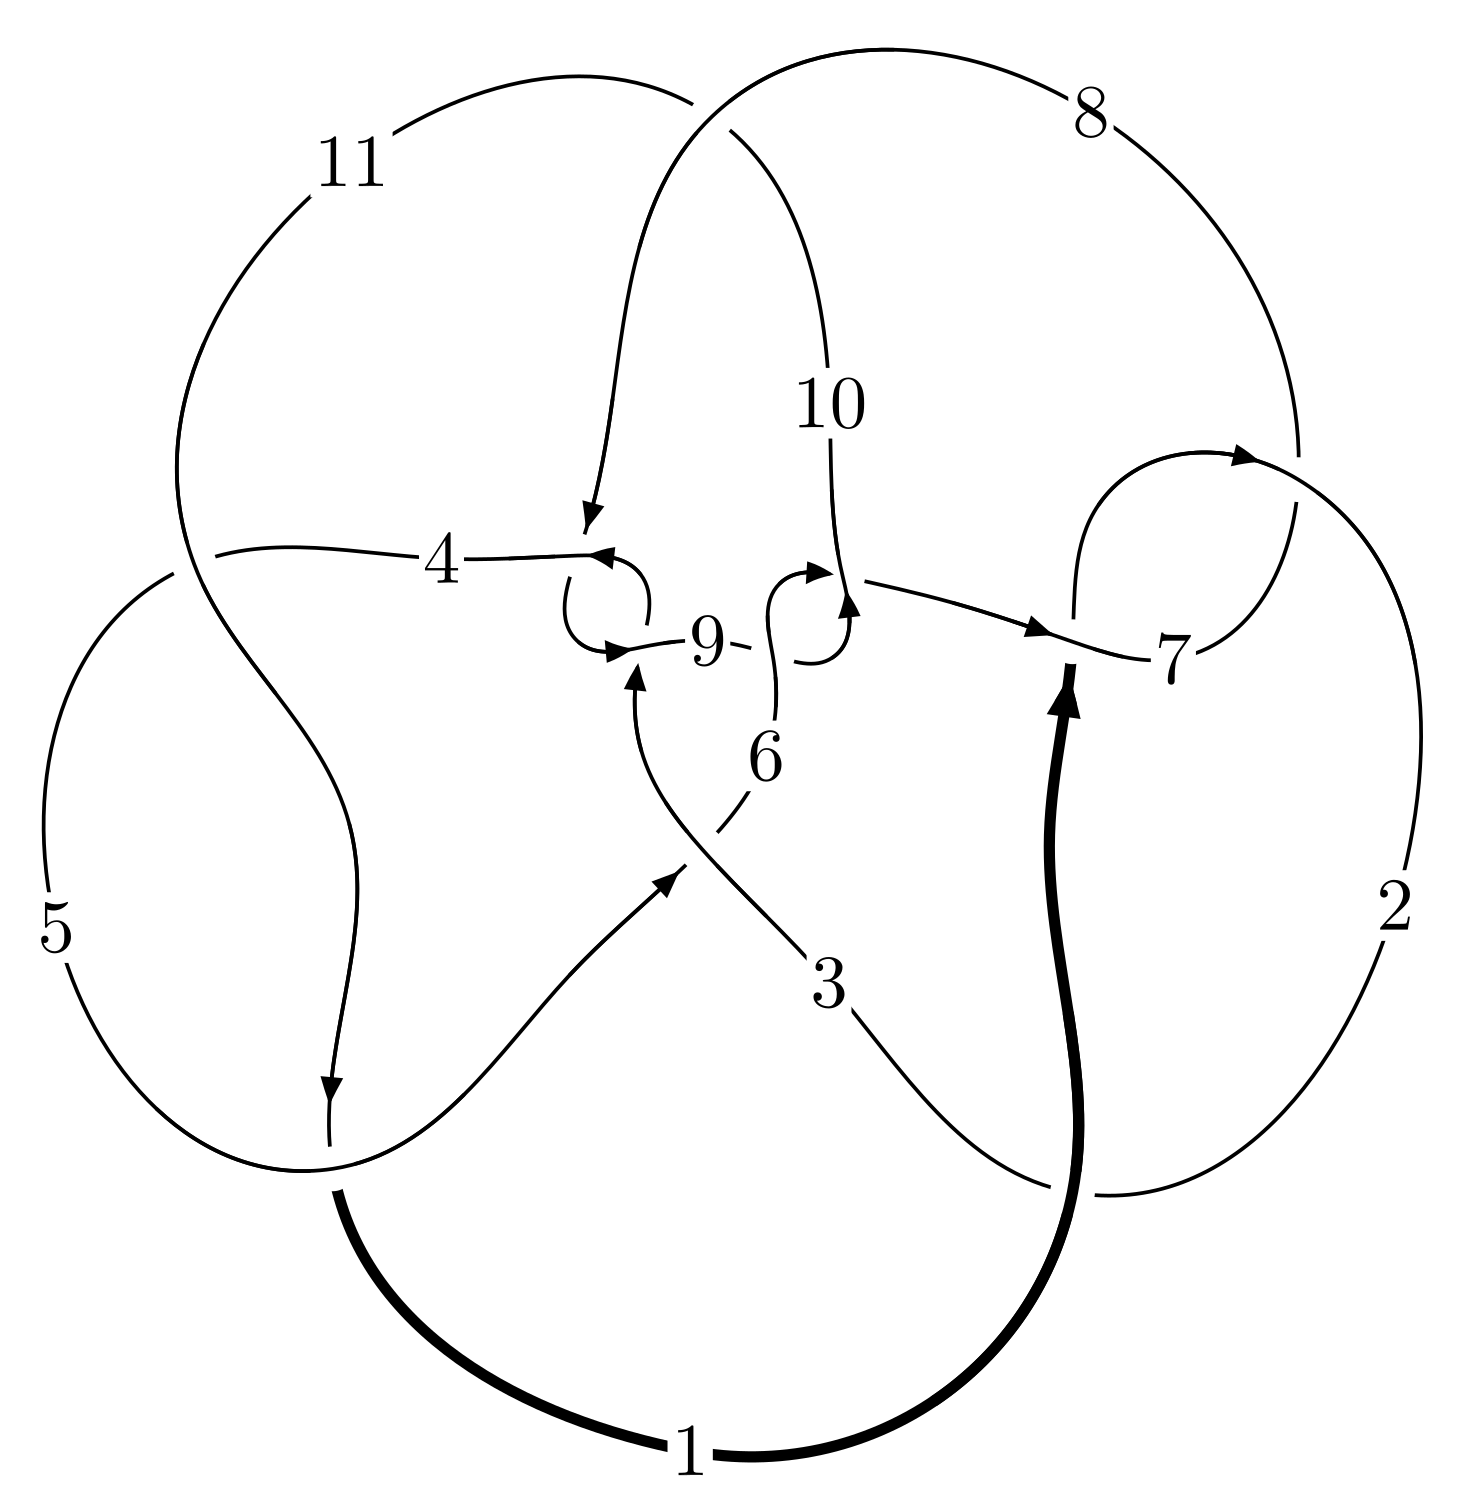
\includegraphics[width=112pt]{../../../GIT/diagram.site/Diagrams/png/481_11a_232.png}\\
\ \ \ A knot diagram\footnotemark}&
\allowdisplaybreaks
\textbf{Linearized knot diagam} \\
\cline{2-2}
 &
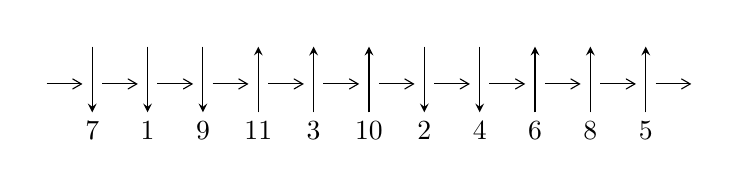
\begin{tikzpicture}[x=20pt, y=17pt]
	% nodes
	\node (C0) at (0, 0) {};
	\node (C1) at (1, 0) {};
	\node (C1U) at (1, +1) {};
	\node (C1D) at (1, -1) {7};

	\node (C2) at (2, 0) {};
	\node (C2U) at (2, +1) {};
	\node (C2D) at (2, -1) {1};

	\node (C3) at (3, 0) {};
	\node (C3U) at (3, +1) {};
	\node (C3D) at (3, -1) {9};

	\node (C4) at (4, 0) {};
	\node (C4U) at (4, +1) {};
	\node (C4D) at (4, -1) {11};

	\node (C5) at (5, 0) {};
	\node (C5U) at (5, +1) {};
	\node (C5D) at (5, -1) {3};

	\node (C6) at (6, 0) {};
	\node (C6U) at (6, +1) {};
	\node (C6D) at (6, -1) {10};

	\node (C7) at (7, 0) {};
	\node (C7U) at (7, +1) {};
	\node (C7D) at (7, -1) {2};

	\node (C8) at (8, 0) {};
	\node (C8U) at (8, +1) {};
	\node (C8D) at (8, -1) {4};

	\node (C9) at (9, 0) {};
	\node (C9U) at (9, +1) {};
	\node (C9D) at (9, -1) {6};

	\node (C10) at (10, 0) {};
	\node (C10U) at (10, +1) {};
	\node (C10D) at (10, -1) {8};

	\node (C11) at (11, 0) {};
	\node (C11U) at (11, +1) {};
	\node (C11D) at (11, -1) {5};
	\node (C12) at (12, 0) {};

	% arrows
	\draw[->,>={angle 60}]
	(C0) edge (C1) (C1) edge (C2) (C2) edge (C3) (C3) edge (C4) (C4) edge (C5) (C5) edge (C6) (C6) edge (C7) (C7) edge (C8) (C8) edge (C9) (C9) edge (C10) (C10) edge (C11) (C11) edge (C12) ;	\draw[->,>=stealth]
	(C1U) edge (C1D) (C2U) edge (C2D) (C3U) edge (C3D) (C4D) edge (C4U) (C5D) edge (C5U) (C6D) edge (C6U) (C7U) edge (C7D) (C8U) edge (C8D) (C9D) edge (C9U) (C10D) edge (C10U) (C11D) edge (C11U) ;
	\end{tikzpicture} \\
\hhline{~~} \\& 
\textbf{Solving Sequence} \\ \cline{2-2} 
 &
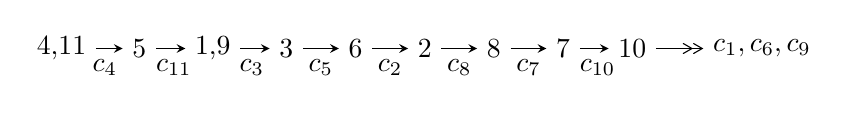
\begin{tikzpicture}[x=25pt, y=7pt]
	% node
	\node (A0) at (-1/8, 0) {4,11};
	\node (A1) at (1, 0) {5};
	\node (A2) at (33/16, 0) {1,9};
	\node (A3) at (25/8, 0) {3};
	\node (A4) at (33/8, 0) {6};
	\node (A5) at (41/8, 0) {2};
	\node (A6) at (49/8, 0) {8};
	\node (A7) at (57/8, 0) {7};
	\node (A8) at (65/8, 0) {10};
	\node (C1) at (1/2, -1) {$c_{4}$};
	\node (C2) at (3/2, -1) {$c_{11}$};
	\node (C3) at (21/8, -1) {$c_{3}$};
	\node (C4) at (29/8, -1) {$c_{5}$};
	\node (C5) at (37/8, -1) {$c_{2}$};
	\node (C6) at (45/8, -1) {$c_{8}$};
	\node (C7) at (53/8, -1) {$c_{7}$};
	\node (C8) at (61/8, -1) {$c_{10}$};
	\node (A9) at (10, 0) {$c_{1},c_{6},c_{9}$};

	% edge
	\draw[->,>=stealth]	
	(A0) edge (A1) (A1) edge (A2) (A2) edge (A3) (A3) edge (A4) (A4) edge (A5) (A5) edge (A6) (A6) edge (A7) (A7) edge (A8) ;
	\draw[->>,>={angle 60}]	
	(A8) edge (A9);
\end{tikzpicture} \\ 

\end{tabular} \\

\footnotetext{
The image of knot diagram is generated by the software ``\textbf{Draw programme}" developed by Andrew Bartholomew(\url{http://www.layer8.co.uk/maths/draw/index.htm\#Running-draw}), where we modified some parts for our purpose(\url{https://github.com/CATsTAILs/LinksPainter}).
}\phantom \\ \newline 
\centering \textbf{Ideals for irreducible components\footnotemark of $X_{\text{par}}$} 
 
\begin{align*}
I^u_{1}&=\langle 
-1.29642\times10^{17} u^{27}-9.84068\times10^{16} u^{26}+\cdots+1.77262\times10^{17} b-9.04547\times10^{17},\\
\phantom{I^u_{1}}&\phantom{= \langle  }8.06637\times10^{17} u^{27}+5.36595\times10^{17} u^{26}+\cdots+7.09049\times10^{17} a+6.30715\times10^{17},\;u^{28}+u^{27}+\cdots+14 u+1\rangle \\
I^u_{2}&=\langle 
8.83675\times10^{38} u^{39}-8.11011\times10^{37} u^{38}+\cdots+1.46509\times10^{38} b-1.09806\times10^{40},\\
\phantom{I^u_{2}}&\phantom{= \langle  }-4.97706\times10^{40} u^{39}+1.13228\times10^{40} u^{38}+\cdots+2.49066\times10^{39} a+8.16831\times10^{41},\\
\phantom{I^u_{2}}&\phantom{= \langle  }u^{40}+u^{39}+\cdots+62 u-17\rangle \\
I^u_{3}&=\langle 
b- u,\;4 a^2+4 a u+2 a+u,\;u^2+1\rangle \\
I^u_{4}&=\langle 
b,\;a+1,\;u-1\rangle \\
I^u_{5}&=\langle 
2 b+3 a-1,\;9 a^2-6 a-7,\;u+1\rangle \\
\\
\end{align*}
\raggedright * 5 irreducible components of $\dim_{\mathbb{C}}=0$, with total 75 representations.\\
\footnotetext{All coefficients of polynomials are rational numbers. But the coefficients are sometimes approximated in decimal forms when there is not enough margin.}
\newpage
\renewcommand{\arraystretch}{1}
\centering \section*{I. $I^u_{1}= \langle -1.30\times10^{17} u^{27}-9.84\times10^{16} u^{26}+\cdots+1.77\times10^{17} b-9.05\times10^{17},\;8.07\times10^{17} u^{27}+5.37\times10^{17} u^{26}+\cdots+7.09\times10^{17} a+6.31\times10^{17},\;u^{28}+u^{27}+\cdots+14 u+1 \rangle$}
\flushleft \textbf{(i) Arc colorings}\\
\begin{tabular}{m{7pt} m{180pt} m{7pt} m{180pt} }
\flushright $a_{4}=$&$\begin{pmatrix}1\\0\end{pmatrix}$ \\
\flushright $a_{11}=$&$\begin{pmatrix}0\\u\end{pmatrix}$ \\
\flushright $a_{5}=$&$\begin{pmatrix}1\\- u^2\end{pmatrix}$ \\
\flushright $a_{1}=$&$\begin{pmatrix}u\\- u^3+u\end{pmatrix}$ \\
\flushright $a_{9}=$&$\begin{pmatrix}-1.13763 u^{27}-0.756780 u^{26}+\cdots-56.2473 u-0.889522\\0.731356 u^{27}+0.555147 u^{26}+\cdots+37.3554 u+5.10287\end{pmatrix}$ \\
\flushright $a_{3}=$&$\begin{pmatrix}-4.73051 u^{27}-4.00227 u^{26}+\cdots-238.602 u-33.2692\\0.00848632 u^{27}-0.147004 u^{26}+\cdots-4.43645 u+0.321958\end{pmatrix}$ \\
\flushright $a_{6}=$&$\begin{pmatrix}3.99376 u^{27}+3.52913 u^{26}+\cdots+207.156 u+31.6346\\0.380852 u^{27}+0.222239 u^{26}+\cdots+15.0373 u+1.13763\end{pmatrix}$ \\
\flushright $a_{2}=$&$\begin{pmatrix}-4.57712 u^{27}-3.99984 u^{26}+\cdots-234.261 u-32.6359\\-0.0116520 u^{27}-0.0162144 u^{26}+\cdots-2.05596 u+0.804312\end{pmatrix}$ \\
\flushright $a_{8}=$&$\begin{pmatrix}-0.406276 u^{27}-0.201633 u^{26}+\cdots-18.8919 u+4.21335\\0.731356 u^{27}+0.555147 u^{26}+\cdots+37.3554 u+5.10287\end{pmatrix}$ \\
\flushright $a_{7}=$&$\begin{pmatrix}3.64578 u^{27}+3.25367 u^{26}+\cdots+189.608 u+30.0323\\0.380288 u^{27}+0.344685 u^{26}+\cdots+18.3337 u+1.71038\end{pmatrix}$ \\
\flushright $a_{10}=$&$\begin{pmatrix}-1.60226 u^{27}-1.25428 u^{26}+\cdots-80.5253 u-4.88328\\0.572743 u^{27}+0.573307 u^{26}+\cdots+33.1611 u+4.72202\end{pmatrix}$\\ \flushright $a_{10}=$&$\begin{pmatrix}-1.60226 u^{27}-1.25428 u^{26}+\cdots-80.5253 u-4.88328\\0.572743 u^{27}+0.573307 u^{26}+\cdots+33.1611 u+4.72202\end{pmatrix}$\\&\end{tabular}
\flushleft \textbf{(ii) Obstruction class $= -1$}\\~\\
\flushleft \textbf{(iii) Cusp Shapes $= \frac{33965909975637527}{11078896897135864} u^{27}+\frac{122607961560954003}{44315587588543456} u^{26}+\cdots+\frac{3170991077588347389}{22157793794271728} u+\frac{1229656491980719955}{44315587588543456}$}\\~\\
\newpage\renewcommand{\arraystretch}{1}
\flushleft \textbf{(iv) u-Polynomials at the component}\newline \\
\begin{tabular}{m{50pt}|m{274pt}}
Crossings & \hspace{64pt}u-Polynomials at each crossing \\
\hline $$\begin{aligned}c_{1},c_{7}\end{aligned}$$&$\begin{aligned}
&u^{28}-3 u^{27}+\cdots+14 u-10
\end{aligned}$\\
\hline $$\begin{aligned}c_{2}\end{aligned}$$&$\begin{aligned}
&u^{28}+13 u^{27}+\cdots-404 u+100
\end{aligned}$\\
\hline $$\begin{aligned}c_{3},c_{8}\end{aligned}$$&$\begin{aligned}
&u^{28}-3 u^{27}+\cdots+170 u-26
\end{aligned}$\\
\hline $$\begin{aligned}c_{4},c_{6},c_{9}\\c_{11}\end{aligned}$$&$\begin{aligned}
&u^{28}- u^{27}+\cdots-14 u+1
\end{aligned}$\\
\hline $$\begin{aligned}c_{5},c_{10}\end{aligned}$$&$\begin{aligned}
&16(16 u^{28}+48 u^{27}+\cdots-4 u-1)
\end{aligned}$\\
\hline
\end{tabular}\\~\\
\newpage\renewcommand{\arraystretch}{1}
\flushleft \textbf{(v) Riley Polynomials at the component}\newline \\
\begin{tabular}{m{50pt}|m{274pt}}
Crossings & \hspace{64pt}Riley Polynomials at each crossing \\
\hline $$\begin{aligned}c_{1},c_{7}\end{aligned}$$&$\begin{aligned}
&y^{28}-13 y^{27}+\cdots+404 y+100
\end{aligned}$\\
\hline $$\begin{aligned}c_{2}\end{aligned}$$&$\begin{aligned}
&y^{28}+7 y^{27}+\cdots-672016 y+10000
\end{aligned}$\\
\hline $$\begin{aligned}c_{3},c_{8}\end{aligned}$$&$\begin{aligned}
&y^{28}+17 y^{27}+\cdots+8332 y+676
\end{aligned}$\\
\hline $$\begin{aligned}c_{4},c_{6},c_{9}\\c_{11}\end{aligned}$$&$\begin{aligned}
&y^{28}-19 y^{27}+\cdots-94 y+1
\end{aligned}$\\
\hline $$\begin{aligned}c_{5},c_{10}\end{aligned}$$&$\begin{aligned}
&256(256 y^{28}-5248 y^{27}+\cdots-74 y+1)
\end{aligned}$\\
\hline
\end{tabular}\\~\\
\newpage\flushleft \textbf{(vi) Complex Volumes and Cusp Shapes}
$$\begin{array}{c|c|c}  
\text{Solutions to }I^u_{1}& \I (\text{vol} + \sqrt{-1}CS) & \text{Cusp shape}\\
 \hline 
\begin{aligned}
u &= -0.449964 + 0.955908 I \\
a &= \phantom{-}0.151228 - 0.563693 I \\
b &= -0.237420 + 1.011880 I\end{aligned}
 & -0.873376 - 0.763619 I & -0.834378 - 1.006413 I \\ \hline\begin{aligned}
u &= -0.449964 - 0.955908 I \\
a &= \phantom{-}0.151228 + 0.563693 I \\
b &= -0.237420 - 1.011880 I\end{aligned}
 & -0.873376 + 0.763619 I & -0.834378 + 1.006413 I \\ \hline\begin{aligned}
u &= \phantom{-}0.619030 + 0.625848 I \\
a &= -0.254904 - 0.940243 I \\
b &= -0.564972 + 0.419726 I\end{aligned}
 & -2.54273 + 3.94340 I & -3.92883 - 8.11948 I \\ \hline\begin{aligned}
u &= \phantom{-}0.619030 - 0.625848 I \\
a &= -0.254904 + 0.940243 I \\
b &= -0.564972 - 0.419726 I\end{aligned}
 & -2.54273 - 3.94340 I & -3.92883 + 8.11948 I \\ \hline\begin{aligned}
u &= \phantom{-}1.16749\phantom{ +0.000000I} \\
a &= \phantom{-}1.09598\phantom{ +0.000000I} \\
b &= -1.79695\phantom{ +0.000000I}\end{aligned}
 & -0.740696\phantom{ +0.000000I} & \phantom{-}13.3630\phantom{ +0.000000I} \\ \hline\begin{aligned}
u &= \phantom{-}0.197638 + 0.798678 I \\
a &= -0.160215 - 0.828722 I \\
b &= -0.165189 + 0.201586 I\end{aligned}
 & -1.59476 - 1.80480 I & -5.09710 + 1.86642 I \\ \hline\begin{aligned}
u &= \phantom{-}0.197638 - 0.798678 I \\
a &= -0.160215 + 0.828722 I \\
b &= -0.165189 - 0.201586 I\end{aligned}
 & -1.59476 + 1.80480 I & -5.09710 - 1.86642 I \\ \hline\begin{aligned}
u &= \phantom{-}0.737049\phantom{ +0.000000I} \\
a &= -0.944844\phantom{ +0.000000I} \\
b &= \phantom{-}1.11268\phantom{ +0.000000I}\end{aligned}
 & -2.48664\phantom{ +0.000000I} & -6.62100\phantom{ +0.000000I} \\ \hline\begin{aligned}
u &= -1.279000 + 0.337291 I \\
a &= -0.47967 + 1.95384 I \\
b &= -0.47948 - 1.61552 I\end{aligned}
 & \phantom{-}5.51780 - 7.86345 I & \phantom{-}5.31743 + 6.29867 I \\ \hline\begin{aligned}
u &= -1.279000 - 0.337291 I \\
a &= -0.47967 - 1.95384 I \\
b &= -0.47948 + 1.61552 I\end{aligned}
 & \phantom{-}5.51780 + 7.86345 I & \phantom{-}5.31743 - 6.29867 I\\
 \hline 
 \end{array}$$\newpage$$\begin{array}{c|c|c}  
\text{Solutions to }I^u_{1}& \I (\text{vol} + \sqrt{-1}CS) & \text{Cusp shape}\\
 \hline 
\begin{aligned}
u &= -1.343250 + 0.043119 I \\
a &= \phantom{-}0.13328 - 1.60960 I \\
b &= -0.76458 + 1.59693 I\end{aligned}
 & \phantom{-}10.03540 - 2.66746 I & \phantom{-}10.12620 + 2.06407 I \\ \hline\begin{aligned}
u &= -1.343250 - 0.043119 I \\
a &= \phantom{-}0.13328 + 1.60960 I \\
b &= -0.76458 - 1.59693 I\end{aligned}
 & \phantom{-}10.03540 + 2.66746 I & \phantom{-}10.12620 - 2.06407 I \\ \hline\begin{aligned}
u &= -1.326140 + 0.226084 I \\
a &= -0.460345 - 0.367905 I \\
b &= \phantom{-}1.374270 + 0.188673 I\end{aligned}
 & \phantom{-}7.76911 - 3.65914 I & \phantom{-}8.46465 + 3.07912 I \\ \hline\begin{aligned}
u &= -1.326140 - 0.226084 I \\
a &= -0.460345 + 0.367905 I \\
b &= \phantom{-}1.374270 - 0.188673 I\end{aligned}
 & \phantom{-}7.76911 + 3.65914 I & \phantom{-}8.46465 - 3.07912 I \\ \hline\begin{aligned}
u &= \phantom{-}1.320310 + 0.365382 I \\
a &= \phantom{-}0.305908 - 0.482073 I \\
b &= -1.262860 + 0.217604 I\end{aligned}
 & \phantom{-}6.13143 + 10.28480 I & \phantom{-}5.46409 - 7.36805 I \\ \hline\begin{aligned}
u &= \phantom{-}1.320310 - 0.365382 I \\
a &= \phantom{-}0.305908 + 0.482073 I \\
b &= -1.262860 - 0.217604 I\end{aligned}
 & \phantom{-}6.13143 - 10.28480 I & \phantom{-}5.46409 + 7.36805 I \\ \hline\begin{aligned}
u &= \phantom{-}1.399260 + 0.113511 I \\
a &= \phantom{-}0.13439 + 1.69651 I \\
b &= \phantom{-}0.64640 - 1.61358 I\end{aligned}
 & \phantom{-}12.33890 + 4.05891 I & \phantom{-}10.87964 - 3.34376 I \\ \hline\begin{aligned}
u &= \phantom{-}1.399260 - 0.113511 I \\
a &= \phantom{-}0.13439 - 1.69651 I \\
b &= \phantom{-}0.64640 + 1.61358 I\end{aligned}
 & \phantom{-}12.33890 - 4.05891 I & \phantom{-}10.87964 + 3.34376 I \\ \hline\begin{aligned}
u &= -0.351747 + 0.453003 I \\
a &= \phantom{-}0.576176 - 0.742859 I \\
b &= \phantom{-}0.246070 + 0.616533 I\end{aligned}
 & \phantom{-}0.183505 - 1.179080 I & \phantom{-}2.03457 + 5.91305 I \\ \hline\begin{aligned}
u &= -0.351747 - 0.453003 I \\
a &= \phantom{-}0.576176 + 0.742859 I \\
b &= \phantom{-}0.246070 - 0.616533 I\end{aligned}
 & \phantom{-}0.183505 + 1.179080 I & \phantom{-}2.03457 - 5.91305 I\\
 \hline 
 \end{array}$$\newpage$$\begin{array}{c|c|c}  
\text{Solutions to }I^u_{1}& \I (\text{vol} + \sqrt{-1}CS) & \text{Cusp shape}\\
 \hline 
\begin{aligned}
u &= \phantom{-}1.47134 + 0.46584 I \\
a &= \phantom{-}0.62737 + 1.64310 I \\
b &= \phantom{-}0.52803 - 1.50973 I\end{aligned}
 & \phantom{-}13.2391 + 10.1973 I & \phantom{-}8.61620 - 4.40012 I \\ \hline\begin{aligned}
u &= \phantom{-}1.47134 - 0.46584 I \\
a &= \phantom{-}0.62737 - 1.64310 I \\
b &= \phantom{-}0.52803 + 1.50973 I\end{aligned}
 & \phantom{-}13.2391 - 10.1973 I & \phantom{-}8.61620 + 4.40012 I \\ \hline\begin{aligned}
u &= -1.45739 + 0.55230 I \\
a &= -0.73550 + 1.62993 I \\
b &= -0.51262 - 1.48286 I\end{aligned}
 & \phantom{-}11.5116 - 16.4523 I & \phantom{-}6.49151 + 8.57137 I \\ \hline\begin{aligned}
u &= -1.45739 - 0.55230 I \\
a &= -0.73550 - 1.62993 I \\
b &= -0.51262 + 1.48286 I\end{aligned}
 & \phantom{-}11.5116 + 16.4523 I & \phantom{-}6.49151 - 8.57137 I \\ \hline\begin{aligned}
u &= -0.11349 + 1.56139 I \\
a &= \phantom{-}0.012320 - 0.622298 I \\
b &= -0.039307 + 1.237680 I\end{aligned}
 & \phantom{-}1.50736 + 2.52809 I & \phantom{-}9.13783 - 4.03367 I \\ \hline\begin{aligned}
u &= -0.11349 - 1.56139 I \\
a &= \phantom{-}0.012320 + 0.622298 I \\
b &= -0.039307 - 1.237680 I\end{aligned}
 & \phantom{-}1.50736 - 2.52809 I & \phantom{-}9.13783 + 4.03367 I \\ \hline\begin{aligned}
u &= -0.138862 + 0.028897 I \\
a &= \phantom{-}6.57439 - 1.46045 I \\
b &= \phantom{-}0.073787 + 0.991855 I\end{aligned}
 & \phantom{-}1.72032 - 2.04511 I & \phantom{-}7.95707 + 3.99629 I \\ \hline\begin{aligned}
u &= -0.138862 - 0.028897 I \\
a &= \phantom{-}6.57439 + 1.46045 I \\
b &= \phantom{-}0.073787 - 0.991855 I\end{aligned}
 & \phantom{-}1.72032 + 2.04511 I & \phantom{-}7.95707 - 3.99629 I\\
 \hline 
 \end{array}$$\newpage\newpage\renewcommand{\arraystretch}{1}
\centering \section*{II. $I^u_{2}= \langle 8.84\times10^{38} u^{39}-8.11\times10^{37} u^{38}+\cdots+1.47\times10^{38} b-1.10\times10^{40},\;-4.98\times10^{40} u^{39}+1.13\times10^{40} u^{38}+\cdots+2.49\times10^{39} a+8.17\times10^{41},\;u^{40}+u^{39}+\cdots+62 u-17 \rangle$}
\flushleft \textbf{(i) Arc colorings}\\
\begin{tabular}{m{7pt} m{180pt} m{7pt} m{180pt} }
\flushright $a_{4}=$&$\begin{pmatrix}1\\0\end{pmatrix}$ \\
\flushright $a_{11}=$&$\begin{pmatrix}0\\u\end{pmatrix}$ \\
\flushright $a_{5}=$&$\begin{pmatrix}1\\- u^2\end{pmatrix}$ \\
\flushright $a_{1}=$&$\begin{pmatrix}u\\- u^3+u\end{pmatrix}$ \\
\flushright $a_{9}=$&$\begin{pmatrix}19.9829 u^{39}-4.54610 u^{38}+\cdots+1425.22 u-327.958\\-6.03152 u^{39}+0.553556 u^{38}+\cdots-361.279 u+74.9478\end{pmatrix}$ \\
\flushright $a_{3}=$&$\begin{pmatrix}-2.14148 u^{39}+1.22331 u^{38}+\cdots-238.675 u+70.6524\\9.32536 u^{39}-1.34018 u^{38}+\cdots+615.450 u-133.266\end{pmatrix}$ \\
\flushright $a_{6}=$&$\begin{pmatrix}42.0817 u^{39}-10.6590 u^{38}+\cdots+3089.04 u-737.735\\-3.20706 u^{39}-0.115380 u^{38}+\cdots-141.669 u+19.2163\end{pmatrix}$ \\
\flushright $a_{2}=$&$\begin{pmatrix}9.46024 u^{39}-0.795742 u^{38}+\cdots+543.626 u-105.550\\5.22480 u^{39}-0.852228 u^{38}+\cdots+356.034 u-77.9153\end{pmatrix}$ \\
\flushright $a_{8}=$&$\begin{pmatrix}13.9514 u^{39}-3.99254 u^{38}+\cdots+1063.94 u-253.010\\-6.03152 u^{39}+0.553556 u^{38}+\cdots-361.279 u+74.9478\end{pmatrix}$ \\
\flushright $a_{7}=$&$\begin{pmatrix}21.9203 u^{39}-3.79830 u^{38}+\cdots+1464.70 u-321.059\\1.20951 u^{39}-0.423156 u^{38}+\cdots+108.425 u-25.8667\end{pmatrix}$ \\
\flushright $a_{10}=$&$\begin{pmatrix}46.8670 u^{39}-4.18670 u^{38}+\cdots+2852.32 u-583.520\\-7.30074 u^{39}+1.70611 u^{38}+\cdots-508.014 u+122.126\end{pmatrix}$\\ \flushright $a_{10}=$&$\begin{pmatrix}46.8670 u^{39}-4.18670 u^{38}+\cdots+2852.32 u-583.520\\-7.30074 u^{39}+1.70611 u^{38}+\cdots-508.014 u+122.126\end{pmatrix}$\\&\end{tabular}
\flushleft \textbf{(ii) Obstruction class $= -1$}\\~\\
\flushleft \textbf{(iii) Cusp Shapes $= 41.4508 u^{39}-6.22688 u^{38}+\cdots+2767.85 u-602.998$}\\~\\
\newpage\renewcommand{\arraystretch}{1}
\flushleft \textbf{(iv) u-Polynomials at the component}\newline \\
\begin{tabular}{m{50pt}|m{274pt}}
Crossings & \hspace{64pt}u-Polynomials at each crossing \\
\hline $$\begin{aligned}c_{1},c_{7}\end{aligned}$$&$\begin{aligned}
&(u^{20}+u^{19}+\cdots+3 u^2-1)^{2}
\end{aligned}$\\
\hline $$\begin{aligned}c_{2}\end{aligned}$$&$\begin{aligned}
&(u^{20}+7 u^{19}+\cdots+6 u+1)^{2}
\end{aligned}$\\
\hline $$\begin{aligned}c_{3},c_{8}\end{aligned}$$&$\begin{aligned}
&(u^{20}+u^{19}+\cdots+2 u-1)^{2}
\end{aligned}$\\
\hline $$\begin{aligned}c_{4},c_{6},c_{9}\\c_{11}\end{aligned}$$&$\begin{aligned}
&u^{40}- u^{39}+\cdots-62 u-17
\end{aligned}$\\
\hline $$\begin{aligned}c_{5},c_{10}\end{aligned}$$&$\begin{aligned}
&u^{40}-5 u^{39}+\cdots-3518 u+8903
\end{aligned}$\\
\hline
\end{tabular}\\~\\
\newpage\renewcommand{\arraystretch}{1}
\flushleft \textbf{(v) Riley Polynomials at the component}\newline \\
\begin{tabular}{m{50pt}|m{274pt}}
Crossings & \hspace{64pt}Riley Polynomials at each crossing \\
\hline $$\begin{aligned}c_{1},c_{7}\end{aligned}$$&$\begin{aligned}
&(y^{20}-7 y^{19}+\cdots-6 y+1)^{2}
\end{aligned}$\\
\hline $$\begin{aligned}c_{2}\end{aligned}$$&$\begin{aligned}
&(y^{20}+13 y^{19}+\cdots-6 y+1)^{2}
\end{aligned}$\\
\hline $$\begin{aligned}c_{3},c_{8}\end{aligned}$$&$\begin{aligned}
&(y^{20}+17 y^{19}+\cdots-6 y+1)^{2}
\end{aligned}$\\
\hline $$\begin{aligned}c_{4},c_{6},c_{9}\\c_{11}\end{aligned}$$&$\begin{aligned}
&y^{40}-29 y^{39}+\cdots-2824 y+289
\end{aligned}$\\
\hline $$\begin{aligned}c_{5},c_{10}\end{aligned}$$&$\begin{aligned}
&y^{40}-25 y^{39}+\cdots-6761242056 y+79263409
\end{aligned}$\\
\hline
\end{tabular}\\~\\
\newpage\flushleft \textbf{(vi) Complex Volumes and Cusp Shapes}
$$\begin{array}{c|c|c}  
\text{Solutions to }I^u_{2}& \I (\text{vol} + \sqrt{-1}CS) & \text{Cusp shape}\\
 \hline 
\begin{aligned}
u &= -1.044840 + 0.243936 I \\
a &= \phantom{-}0.43981 + 1.65317 I \\
b &= -0.201509 + 0.663357 I\end{aligned}
 & \phantom{-}4.95641 + 2.35832 I & \phantom{-}5.64775 - 4.49783 I \\ \hline\begin{aligned}
u &= -1.044840 - 0.243936 I \\
a &= \phantom{-}0.43981 - 1.65317 I \\
b &= -0.201509 - 0.663357 I\end{aligned}
 & \phantom{-}4.95641 - 2.35832 I & \phantom{-}5.64775 + 4.49783 I \\ \hline\begin{aligned}
u &= \phantom{-}1.101170 + 0.208325 I \\
a &= -2.01145 + 0.48533 I \\
b &= -0.201509 + 0.663357 I\end{aligned}
 & \phantom{-}4.95641 + 2.35832 I & \phantom{-}5.64775 - 4.49783 I \\ \hline\begin{aligned}
u &= \phantom{-}1.101170 - 0.208325 I \\
a &= -2.01145 - 0.48533 I \\
b &= -0.201509 - 0.663357 I\end{aligned}
 & \phantom{-}4.95641 - 2.35832 I & \phantom{-}5.64775 + 4.49783 I \\ \hline\begin{aligned}
u &= -1.13898\phantom{ +0.000000I} \\
a &= \phantom{-}0.459946\phantom{ +0.000000I} \\
b &= -0.358818\phantom{ +0.000000I}\end{aligned}
 & \phantom{-}2.60969\phantom{ +0.000000I} & -2.76210\phantom{ +0.000000I} \\ \hline\begin{aligned}
u &= -1.156830 + 0.007308 I \\
a &= \phantom{-}1.56319 + 2.12053 I \\
b &= \phantom{-}0.274747 - 1.069600 I\end{aligned}
 & \phantom{-}4.55875 - 2.13456 I & \phantom{-}3.49102 + 2.16962 I \\ \hline\begin{aligned}
u &= -1.156830 - 0.007308 I \\
a &= \phantom{-}1.56319 - 2.12053 I \\
b &= \phantom{-}0.274747 + 1.069600 I\end{aligned}
 & \phantom{-}4.55875 + 2.13456 I & \phantom{-}3.49102 - 2.16962 I \\ \hline\begin{aligned}
u &= -0.598773 + 0.548760 I \\
a &= -1.130270 - 0.298739 I \\
b &= -0.198534 - 1.239650 I\end{aligned}
 & \phantom{-}6.05405 - 2.16136 I & \phantom{-}7.26252 + 3.31855 I \\ \hline\begin{aligned}
u &= -0.598773 - 0.548760 I \\
a &= -1.130270 + 0.298739 I \\
b &= -0.198534 + 1.239650 I\end{aligned}
 & \phantom{-}6.05405 + 2.16136 I & \phantom{-}7.26252 - 3.31855 I \\ \hline\begin{aligned}
u &= -0.059958 + 0.789733 I \\
a &= \phantom{-}0.671566 + 0.796017 I \\
b &= \phantom{-}0.773104 + 0.153161 I\end{aligned}
 & \phantom{-}1.80703 - 6.07240 I & \phantom{-}0.54715 + 5.87540 I\\
 \hline 
 \end{array}$$\newpage$$\begin{array}{c|c|c}  
\text{Solutions to }I^u_{2}& \I (\text{vol} + \sqrt{-1}CS) & \text{Cusp shape}\\
 \hline 
\begin{aligned}
u &= -0.059958 - 0.789733 I \\
a &= \phantom{-}0.671566 - 0.796017 I \\
b &= \phantom{-}0.773104 - 0.153161 I\end{aligned}
 & \phantom{-}1.80703 + 6.07240 I & \phantom{-}0.54715 - 5.87540 I \\ \hline\begin{aligned}
u &= -1.151180 + 0.376978 I \\
a &= \phantom{-}0.78707 - 1.80536 I \\
b &= \phantom{-}0.327541 + 1.260030 I\end{aligned}
 & \phantom{-}1.63329 - 3.96853 I & \phantom{-0.000000 -}0. + 3.79787 I \\ \hline\begin{aligned}
u &= -1.151180 - 0.376978 I \\
a &= \phantom{-}0.78707 + 1.80536 I \\
b &= \phantom{-}0.327541 - 1.260030 I\end{aligned}
 & \phantom{-}1.63329 + 3.96853 I & \phantom{-0.000000 } 0. - 3.79787 I \\ \hline\begin{aligned}
u &= -0.265136 + 1.197750 I \\
a &= -0.299881 + 0.427278 I \\
b &= -0.295567 - 1.352050 I\end{aligned}
 & \phantom{-}7.72048 - 4.43308 I & \phantom{-}7.31630 + 0. I\phantom{ +0.000000I} \\ \hline\begin{aligned}
u &= -0.265136 - 1.197750 I \\
a &= -0.299881 - 0.427278 I \\
b &= -0.295567 + 1.352050 I\end{aligned}
 & \phantom{-}7.72048 + 4.43308 I & \phantom{-}7.31630 + 0. I\phantom{ +0.000000I} \\ \hline\begin{aligned}
u &= -1.219460 + 0.187157 I \\
a &= \phantom{-}0.0698643 - 0.0332146 I \\
b &= -0.692333 - 0.156175 I\end{aligned}
 & \phantom{-}2.96536 - 0.81573 I & \phantom{-0.000000 } 0 \\ \hline\begin{aligned}
u &= -1.219460 - 0.187157 I \\
a &= \phantom{-}0.0698643 + 0.0332146 I \\
b &= -0.692333 + 0.156175 I\end{aligned}
 & \phantom{-}2.96536 + 0.81573 I & \phantom{-0.000000 } 0 \\ \hline\begin{aligned}
u &= \phantom{-}0.733960\phantom{ +0.000000I} \\
a &= -1.52495\phantom{ +0.000000I} \\
b &= -0.358818\phantom{ +0.000000I}\end{aligned}
 & \phantom{-}2.60969\phantom{ +0.000000I} & -2.76210\phantom{ +0.000000I} \\ \hline\begin{aligned}
u &= \phantom{-}0.616504 + 0.374474 I \\
a &= -0.258415 + 0.450813 I \\
b &= \phantom{-}0.772326\phantom{ +0.000000I}\end{aligned}
 & -2.26801\phantom{ +0.000000I} & -4.44026 + 0. I\phantom{ +0.000000I} \\ \hline\begin{aligned}
u &= \phantom{-}0.616504 - 0.374474 I \\
a &= -0.258415 - 0.450813 I \\
b &= \phantom{-}0.772326\phantom{ +0.000000I}\end{aligned}
 & -2.26801\phantom{ +0.000000I} & -4.44026 + 0. I\phantom{ +0.000000I}\\
 \hline 
 \end{array}$$\newpage$$\begin{array}{c|c|c}  
\text{Solutions to }I^u_{2}& \I (\text{vol} + \sqrt{-1}CS) & \text{Cusp shape}\\
 \hline 
\begin{aligned}
u &= -0.046221 + 0.711923 I \\
a &= -0.345881 + 0.305536 I \\
b &= \phantom{-}0.327541 - 1.260030 I\end{aligned}
 & \phantom{-}1.63329 + 3.96853 I & \phantom{-}0.10651 - 3.79787 I \\ \hline\begin{aligned}
u &= -0.046221 - 0.711923 I \\
a &= -0.345881 - 0.305536 I \\
b &= \phantom{-}0.327541 + 1.260030 I\end{aligned}
 & \phantom{-}1.63329 - 3.96853 I & \phantom{-}0.10651 + 3.79787 I \\ \hline\begin{aligned}
u &= \phantom{-}0.094315 + 1.289960 I \\
a &= \phantom{-}0.241791 + 0.504558 I \\
b &= \phantom{-}0.328206 - 1.357610 I\end{aligned}
 & \phantom{-}6.57229 + 10.05770 I & \phantom{-0.000000 } 0 \\ \hline\begin{aligned}
u &= \phantom{-}0.094315 - 1.289960 I \\
a &= \phantom{-}0.241791 - 0.504558 I \\
b &= \phantom{-}0.328206 + 1.357610 I\end{aligned}
 & \phantom{-}6.57229 - 10.05770 I & \phantom{-0.000000 } 0 \\ \hline\begin{aligned}
u &= \phantom{-}1.240730 + 0.365535 I \\
a &= \phantom{-}0.0134609 + 0.0435217 I \\
b &= \phantom{-}0.773104 - 0.153161 I\end{aligned}
 & \phantom{-}1.80703 + 6.07240 I & \phantom{-0.000000 } 0 \\ \hline\begin{aligned}
u &= \phantom{-}1.240730 - 0.365535 I \\
a &= \phantom{-}0.0134609 - 0.0435217 I \\
b &= \phantom{-}0.773104 + 0.153161 I\end{aligned}
 & \phantom{-}1.80703 - 6.07240 I & \phantom{-0.000000 } 0 \\ \hline\begin{aligned}
u &= \phantom{-}1.307700 + 0.029974 I \\
a &= -0.28588 - 2.24493 I \\
b &= -0.198534 + 1.239650 I\end{aligned}
 & \phantom{-}6.05405 + 2.16136 I & \phantom{-0.000000 } 0 \\ \hline\begin{aligned}
u &= \phantom{-}1.307700 - 0.029974 I \\
a &= -0.28588 + 2.24493 I \\
b &= -0.198534 - 1.239650 I\end{aligned}
 & \phantom{-}6.05405 - 2.16136 I & \phantom{-0.000000 } 0 \\ \hline\begin{aligned}
u &= \phantom{-}0.245936 + 0.564099 I \\
a &= -1.06678 + 0.97261 I \\
b &= -0.692333 + 0.156175 I\end{aligned}
 & \phantom{-}2.96536 + 0.81573 I & \phantom{-}2.32828 - 1.07888 I \\ \hline\begin{aligned}
u &= \phantom{-}0.245936 - 0.564099 I \\
a &= -1.06678 - 0.97261 I \\
b &= -0.692333 - 0.156175 I\end{aligned}
 & \phantom{-}2.96536 - 0.81573 I & \phantom{-}2.32828 + 1.07888 I\\
 \hline 
 \end{array}$$\newpage$$\begin{array}{c|c|c}  
\text{Solutions to }I^u_{2}& \I (\text{vol} + \sqrt{-1}CS) & \text{Cusp shape}\\
 \hline 
\begin{aligned}
u &= \phantom{-}0.509345 + 0.095450 I \\
a &= \phantom{-}2.70967 + 2.44353 I \\
b &= \phantom{-}0.274747 + 1.069600 I\end{aligned}
 & \phantom{-}4.55875 + 2.13456 I & \phantom{-}3.49102 - 2.16962 I \\ \hline\begin{aligned}
u &= \phantom{-}0.509345 - 0.095450 I \\
a &= \phantom{-}2.70967 - 2.44353 I \\
b &= \phantom{-}0.274747 - 1.069600 I\end{aligned}
 & \phantom{-}4.55875 - 2.13456 I & \phantom{-}3.49102 + 2.16962 I \\ \hline\begin{aligned}
u &= \phantom{-}1.56466 + 0.43256 I \\
a &= -0.46583 - 1.54438 I \\
b &= -0.295567 + 1.352050 I\end{aligned}
 & \phantom{-}7.72048 + 4.43308 I & \phantom{-0.000000 } 0 \\ \hline\begin{aligned}
u &= \phantom{-}1.56466 - 0.43256 I \\
a &= -0.46583 + 1.54438 I \\
b &= -0.295567 - 1.352050 I\end{aligned}
 & \phantom{-}7.72048 - 4.43308 I & \phantom{-0.000000 } 0 \\ \hline\begin{aligned}
u &= -1.54550 + 0.58408 I \\
a &= \phantom{-}0.55643 - 1.46280 I \\
b &= \phantom{-}0.328206 + 1.357610 I\end{aligned}
 & \phantom{-}6.57229 - 10.05770 I & \phantom{-0.000000 } 0 \\ \hline\begin{aligned}
u &= -1.54550 - 0.58408 I \\
a &= \phantom{-}0.55643 + 1.46280 I \\
b &= \phantom{-}0.328206 - 1.357610 I\end{aligned}
 & \phantom{-}6.57229 + 10.05770 I & \phantom{-0.000000 } 0 \\ \hline\begin{aligned}
u &= -1.48897 + 0.75285 I \\
a &= -0.601546 + 1.129320 I \\
b &= -0.022410 - 1.403750 I\end{aligned}
 & \phantom{-}11.26460 - 2.84648 I & \phantom{-0.000000 } 0 \\ \hline\begin{aligned}
u &= -1.48897 - 0.75285 I \\
a &= -0.601546 - 1.129320 I \\
b &= -0.022410 + 1.403750 I\end{aligned}
 & \phantom{-}11.26460 + 2.84648 I & \phantom{-0.000000 } 0 \\ \hline\begin{aligned}
u &= \phantom{-}1.59903 + 0.60741 I \\
a &= \phantom{-}0.504411 + 1.265840 I \\
b &= -0.022410 - 1.403750 I\end{aligned}
 & \phantom{-}11.26460 - 2.84648 I & \phantom{-0.000000 } 0 \\ \hline\begin{aligned}
u &= \phantom{-}1.59903 - 0.60741 I \\
a &= \phantom{-}0.504411 - 1.265840 I \\
b &= -0.022410 + 1.403750 I\end{aligned}
 & \phantom{-}11.26460 + 2.84648 I & \phantom{-0.000000 } 0\\
 \hline 
 \end{array}$$\newpage\newpage\renewcommand{\arraystretch}{1}
\centering \section*{III. $I^u_{3}= \langle b- u,\;4 a^2+4 a u+2 a+u,\;u^2+1 \rangle$}
\flushleft \textbf{(i) Arc colorings}\\
\begin{tabular}{m{7pt} m{180pt} m{7pt} m{180pt} }
\flushright $a_{4}=$&$\begin{pmatrix}1\\0\end{pmatrix}$ \\
\flushright $a_{11}=$&$\begin{pmatrix}0\\u\end{pmatrix}$ \\
\flushright $a_{5}=$&$\begin{pmatrix}1\\1\end{pmatrix}$ \\
\flushright $a_{1}=$&$\begin{pmatrix}u\\2 u\end{pmatrix}$ \\
\flushright $a_{9}=$&$\begin{pmatrix}a\\u\end{pmatrix}$ \\
\flushright $a_{3}=$&$\begin{pmatrix}- a u+1\\1\end{pmatrix}$ \\
\flushright $a_{6}=$&$\begin{pmatrix}\frac{1}{2} a+\frac{1}{4} u+1\\- a u+1\end{pmatrix}$ \\
\flushright $a_{2}=$&$\begin{pmatrix}-3 a u+2\\-4 a u+3\end{pmatrix}$ \\
\flushright $a_{8}=$&$\begin{pmatrix}a+u\\u\end{pmatrix}$ \\
\flushright $a_{7}=$&$\begin{pmatrix}- a u+a+\frac{1}{2} u+2\\-2 a u+3\end{pmatrix}$ \\
\flushright $a_{10}=$&$\begin{pmatrix}\frac{1}{2} a u+a+u-\frac{1}{4}\\a+2 u\end{pmatrix}$\\ \flushright $a_{10}=$&$\begin{pmatrix}\frac{1}{2} a u+a+u-\frac{1}{4}\\a+2 u\end{pmatrix}$\\&\end{tabular}
\flushleft \textbf{(ii) Obstruction class $= 1$}\\~\\
\flushleft \textbf{(iii) Cusp Shapes $= -8 a-4 u$}\\~\\
\newpage\renewcommand{\arraystretch}{1}
\flushleft \textbf{(iv) u-Polynomials at the component}\newline \\
\begin{tabular}{m{50pt}|m{274pt}}
Crossings & \hspace{64pt}u-Polynomials at each crossing \\
\hline $$\begin{aligned}c_{1},c_{7}\end{aligned}$$&$\begin{aligned}
&u^4- u^2+1
\end{aligned}$\\
\hline $$\begin{aligned}c_{2}\end{aligned}$$&$\begin{aligned}
&(u^2+u+1)^2
\end{aligned}$\\
\hline $$\begin{aligned}c_{3},c_{4},c_{6}\\c_{8},c_{9},c_{11}\end{aligned}$$&$\begin{aligned}
&(u^2+1)^2
\end{aligned}$\\
\hline $$\begin{aligned}c_{5},c_{10}\end{aligned}$$&$\begin{aligned}
&16(16 u^4-32 u^3+20 u^2-4 u+1)
\end{aligned}$\\
\hline
\end{tabular}\\~\\
\newpage\renewcommand{\arraystretch}{1}
\flushleft \textbf{(v) Riley Polynomials at the component}\newline \\
\begin{tabular}{m{50pt}|m{274pt}}
Crossings & \hspace{64pt}Riley Polynomials at each crossing \\
\hline $$\begin{aligned}c_{1},c_{7}\end{aligned}$$&$\begin{aligned}
&(y^2- y+1)^2
\end{aligned}$\\
\hline $$\begin{aligned}c_{2}\end{aligned}$$&$\begin{aligned}
&(y^2+y+1)^2
\end{aligned}$\\
\hline $$\begin{aligned}c_{3},c_{4},c_{6}\\c_{8},c_{9},c_{11}\end{aligned}$$&$\begin{aligned}
&(y+1)^4
\end{aligned}$\\
\hline $$\begin{aligned}c_{5},c_{10}\end{aligned}$$&$\begin{aligned}
&256(256 y^4-384 y^3+176 y^2+24 y+1)
\end{aligned}$\\
\hline
\end{tabular}\\~\\
\newpage\flushleft \textbf{(vi) Complex Volumes and Cusp Shapes}
$$\begin{array}{c|c|c}  
\text{Solutions to }I^u_{3}& \I (\text{vol} + \sqrt{-1}CS) & \text{Cusp shape}\\
 \hline 
\begin{aligned}
u &= \phantom{-0.000000 -}1.000000 I \\
a &= -0.250000 - 0.933013 I \\
b &= \phantom{-0.000000 -}1.000000 I\end{aligned}
 & \phantom{-0.000000 } -2.02988 I & \phantom{-}2.00000 + 3.46410 I \\ \hline\begin{aligned}
u &= \phantom{-0.000000 -}1.000000 I \\
a &= -0.250000 - 0.066987 I \\
b &= \phantom{-0.000000 -}1.000000 I\end{aligned}
 & \phantom{-0.000000 -}2.02988 I & \phantom{-}2.00000 - 3.46410 I \\ \hline\begin{aligned}
u &= \phantom{-0.000000 } -1.000000 I \\
a &= -0.250000 + 0.933013 I \\
b &= \phantom{-0.000000 } -1.000000 I\end{aligned}
 & \phantom{-0.000000 -}2.02988 I & \phantom{-}2.00000 - 3.46410 I \\ \hline\begin{aligned}
u &= \phantom{-0.000000 } -1.000000 I \\
a &= -0.250000 + 0.066987 I \\
b &= \phantom{-0.000000 } -1.000000 I\end{aligned}
 & \phantom{-0.000000 } -2.02988 I & \phantom{-}2.00000 + 3.46410 I\\
 \hline 
 \end{array}$$\newpage\newpage\renewcommand{\arraystretch}{1}
\centering \section*{IV. $I^u_{4}= \langle b,\;a+1,\;u-1 \rangle$}
\flushleft \textbf{(i) Arc colorings}\\
\begin{tabular}{m{7pt} m{180pt} m{7pt} m{180pt} }
\flushright $a_{4}=$&$\begin{pmatrix}1\\0\end{pmatrix}$ \\
\flushright $a_{11}=$&$\begin{pmatrix}0\\1\end{pmatrix}$ \\
\flushright $a_{5}=$&$\begin{pmatrix}1\\-1\end{pmatrix}$ \\
\flushright $a_{1}=$&$\begin{pmatrix}1\\0\end{pmatrix}$ \\
\flushright $a_{9}=$&$\begin{pmatrix}-1\\0\end{pmatrix}$ \\
\flushright $a_{3}=$&$\begin{pmatrix}1\\0\end{pmatrix}$ \\
\flushright $a_{6}=$&$\begin{pmatrix}0\\-1\end{pmatrix}$ \\
\flushright $a_{2}=$&$\begin{pmatrix}1\\0\end{pmatrix}$ \\
\flushright $a_{8}=$&$\begin{pmatrix}-1\\0\end{pmatrix}$ \\
\flushright $a_{7}=$&$\begin{pmatrix}-1\\0\end{pmatrix}$ \\
\flushright $a_{10}=$&$\begin{pmatrix}-1\\1\end{pmatrix}$\\ \flushright $a_{10}=$&$\begin{pmatrix}-1\\1\end{pmatrix}$\\&\end{tabular}
\flushleft \textbf{(ii) Obstruction class $= 1$}\\~\\
\flushleft \textbf{(iii) Cusp Shapes $= 12$}\\~\\
\newpage\renewcommand{\arraystretch}{1}
\flushleft \textbf{(iv) u-Polynomials at the component}\newline \\
\begin{tabular}{m{50pt}|m{274pt}}
Crossings & \hspace{64pt}u-Polynomials at each crossing \\
\hline $$\begin{aligned}c_{1},c_{2},c_{3}\\c_{7},c_{8}\end{aligned}$$&$\begin{aligned}
&u
\end{aligned}$\\
\hline $$\begin{aligned}c_{4},c_{5},c_{9}\\c_{10}\end{aligned}$$&$\begin{aligned}
&u-1
\end{aligned}$\\
\hline $$\begin{aligned}c_{6},c_{11}\end{aligned}$$&$\begin{aligned}
&u+1
\end{aligned}$\\
\hline
\end{tabular}\\~\\
\newpage\renewcommand{\arraystretch}{1}
\flushleft \textbf{(v) Riley Polynomials at the component}\newline \\
\begin{tabular}{m{50pt}|m{274pt}}
Crossings & \hspace{64pt}Riley Polynomials at each crossing \\
\hline $$\begin{aligned}c_{1},c_{2},c_{3}\\c_{7},c_{8}\end{aligned}$$&$\begin{aligned}
&y
\end{aligned}$\\
\hline $$\begin{aligned}c_{4},c_{5},c_{6}\\c_{9},c_{10},c_{11}\end{aligned}$$&$\begin{aligned}
&y-1
\end{aligned}$\\
\hline
\end{tabular}\\~\\
\newpage\flushleft \textbf{(vi) Complex Volumes and Cusp Shapes}
$$\begin{array}{c|c|c}  
\text{Solutions to }I^u_{4}& \I (\text{vol} + \sqrt{-1}CS) & \text{Cusp shape}\\
 \hline 
\begin{aligned}
u &= \phantom{-}1.00000\phantom{ +0.000000I} \\
a &= -1.00000\phantom{ +0.000000I} \\
b &= \phantom{-0.000000 } 0\end{aligned}
 & \phantom{-}3.28987\phantom{ +0.000000I} & \phantom{-}12.0000\phantom{ +0.000000I}\\
 \hline 
 \end{array}$$\newpage\newpage\renewcommand{\arraystretch}{1}
\centering \section*{V. $I^u_{5}= \langle 2 b+3 a-1,\;9 a^2-6 a-7,\;u+1 \rangle$}
\flushleft \textbf{(i) Arc colorings}\\
\begin{tabular}{m{7pt} m{180pt} m{7pt} m{180pt} }
\flushright $a_{4}=$&$\begin{pmatrix}1\\0\end{pmatrix}$ \\
\flushright $a_{11}=$&$\begin{pmatrix}0\\-1\end{pmatrix}$ \\
\flushright $a_{5}=$&$\begin{pmatrix}1\\-1\end{pmatrix}$ \\
\flushright $a_{1}=$&$\begin{pmatrix}-1\\0\end{pmatrix}$ \\
\flushright $a_{9}=$&$\begin{pmatrix}a\\-\frac{3}{2} a+\frac{1}{2}\end{pmatrix}$ \\
\flushright $a_{3}=$&$\begin{pmatrix}\frac{1}{2} a+\frac{13}{6}\\-2\end{pmatrix}$ \\
\flushright $a_{6}=$&$\begin{pmatrix}-\frac{4}{3} a+\frac{4}{9}\\a-\frac{2}{3}\end{pmatrix}$ \\
\flushright $a_{2}=$&$\begin{pmatrix}\frac{1}{2} a+\frac{1}{6}\\-2\end{pmatrix}$ \\
\flushright $a_{8}=$&$\begin{pmatrix}-\frac{1}{2} a+\frac{1}{2}\\-\frac{3}{2} a+\frac{1}{2}\end{pmatrix}$ \\
\flushright $a_{7}=$&$\begin{pmatrix}- a\\\frac{3}{2} a-\frac{1}{2}\end{pmatrix}$ \\
\flushright $a_{10}=$&$\begin{pmatrix}-\frac{1}{3} a+\frac{4}{9}\\-\frac{1}{2} a-\frac{1}{6}\end{pmatrix}$\\ \flushright $a_{10}=$&$\begin{pmatrix}-\frac{1}{3} a+\frac{4}{9}\\-\frac{1}{2} a-\frac{1}{6}\end{pmatrix}$\\&\end{tabular}
\flushleft \textbf{(ii) Obstruction class $= 1$}\\~\\
\flushleft \textbf{(iii) Cusp Shapes $= 4$}\\~\\
\newpage\renewcommand{\arraystretch}{1}
\flushleft \textbf{(iv) u-Polynomials at the component}\newline \\
\begin{tabular}{m{50pt}|m{274pt}}
Crossings & \hspace{64pt}u-Polynomials at each crossing \\
\hline $$\begin{aligned}c_{1},c_{3},c_{7}\\c_{8}\end{aligned}$$&$\begin{aligned}
&u^2-2
\end{aligned}$\\
\hline $$\begin{aligned}c_{2}\end{aligned}$$&$\begin{aligned}
&(u+2)^2
\end{aligned}$\\
\hline $$\begin{aligned}c_{4},c_{9}\end{aligned}$$&$\begin{aligned}
&(u+1)^2
\end{aligned}$\\
\hline $$\begin{aligned}c_{5},c_{10}\end{aligned}$$&$\begin{aligned}
&9(9 u^2-6 u-1)
\end{aligned}$\\
\hline $$\begin{aligned}c_{6},c_{11}\end{aligned}$$&$\begin{aligned}
&(u-1)^2
\end{aligned}$\\
\hline
\end{tabular}\\~\\
\newpage\renewcommand{\arraystretch}{1}
\flushleft \textbf{(v) Riley Polynomials at the component}\newline \\
\begin{tabular}{m{50pt}|m{274pt}}
Crossings & \hspace{64pt}Riley Polynomials at each crossing \\
\hline $$\begin{aligned}c_{1},c_{3},c_{7}\\c_{8}\end{aligned}$$&$\begin{aligned}
&(y-2)^2
\end{aligned}$\\
\hline $$\begin{aligned}c_{2}\end{aligned}$$&$\begin{aligned}
&(y-4)^2
\end{aligned}$\\
\hline $$\begin{aligned}c_{4},c_{6},c_{9}\\c_{11}\end{aligned}$$&$\begin{aligned}
&(y-1)^2
\end{aligned}$\\
\hline $$\begin{aligned}c_{5},c_{10}\end{aligned}$$&$\begin{aligned}
&81(81 y^2-54 y+1)
\end{aligned}$\\
\hline
\end{tabular}\\~\\
\newpage\flushleft \textbf{(vi) Complex Volumes and Cusp Shapes}
$$\begin{array}{c|c|c}  
\text{Solutions to }I^u_{5}& \I (\text{vol} + \sqrt{-1}CS) & \text{Cusp shape}\\
 \hline 
\begin{aligned}
u &= -1.00000\phantom{ +0.000000I} \\
a &= \phantom{-}1.27614\phantom{ +0.000000I} \\
b &= -1.41421\phantom{ +0.000000I}\end{aligned}
 & -1.64493\phantom{ +0.000000I} & \phantom{-}4.00000\phantom{ +0.000000I} \\ \hline\begin{aligned}
u &= -1.00000\phantom{ +0.000000I} \\
a &= -0.609476\phantom{ +0.000000I} \\
b &= \phantom{-}1.41421\phantom{ +0.000000I}\end{aligned}
 & -1.64493\phantom{ +0.000000I} & \phantom{-}4.00000\phantom{ +0.000000I}\\
 \hline 
 \end{array}$$\newpage
\newpage\renewcommand{\arraystretch}{1}
\centering \section*{ VI. u-Polynomials}
\begin{tabular}{m{50pt}|m{274pt}}
Crossings & \hspace{64pt}u-Polynomials at each crossing \\
\hline $$\begin{aligned}c_{1},c_{7}\end{aligned}$$&$\begin{aligned}
&u(u^2-2)(u^4- u^2+1)(u^{20}+u^{19}+\cdots+3 u^{2}-1)^{2}\\
&\cdot(u^{28}-3 u^{27}+\cdots+14 u-10)
\end{aligned}$\\
\hline $$\begin{aligned}c_{2}\end{aligned}$$&$\begin{aligned}
&u(u+2)^2(u^2+u+1)^2(u^{20}+7 u^{19}+\cdots+6 u+1)^{2}\\
&\cdot(u^{28}+13 u^{27}+\cdots-404 u+100)
\end{aligned}$\\
\hline $$\begin{aligned}c_{3},c_{8}\end{aligned}$$&$\begin{aligned}
&u(u^2-2)(u^2+1)^2(u^{20}+u^{19}+\cdots+2 u-1)^{2}\\
&\cdot(u^{28}-3 u^{27}+\cdots+170 u-26)
\end{aligned}$\\
\hline $$\begin{aligned}c_{4},c_{9}\end{aligned}$$&$\begin{aligned}
&(u-1)(u+1)^2(u^2+1)^2(u^{28}-u^{27}+\cdots-14 u+1)\\
&\cdot(u^{40}- u^{39}+\cdots-62 u-17)
\end{aligned}$\\
\hline $$\begin{aligned}c_{5},c_{10}\end{aligned}$$&$\begin{aligned}
&2304(u-1)(9 u^2-6 u-1)(16 u^4-32 u^3+20 u^2-4 u+1)\\
&\cdot(16 u^{28}+48 u^{27}+\cdots-4 u-1)(u^{40}-5 u^{39}+\cdots-3518 u+8903)
\end{aligned}$\\
\hline $$\begin{aligned}c_{6},c_{11}\end{aligned}$$&$\begin{aligned}
&((u-1)^2)(u+1)(u^2+1)^2(u^{28}-u^{27}+\cdots-14 u+1)\\
&\cdot(u^{40}- u^{39}+\cdots-62 u-17)
\end{aligned}$\\
\hline
\end{tabular}\newpage\renewcommand{\arraystretch}{1}
\centering \section*{ VII. Riley Polynomials}
\begin{tabular}{m{50pt}|m{274pt}}
Crossings & \hspace{64pt}Riley Polynomials at each crossing \\
\hline $$\begin{aligned}c_{1},c_{7}\end{aligned}$$&$\begin{aligned}
&y(y-2)^2(y^2- y+1)^2(y^{20}-7 y^{19}+\cdots-6 y+1)^{2}\\
&\cdot(y^{28}-13 y^{27}+\cdots+404 y+100)
\end{aligned}$\\
\hline $$\begin{aligned}c_{2}\end{aligned}$$&$\begin{aligned}
&y(y-4)^2(y^2+y+1)^2(y^{20}+13 y^{19}+\cdots-6 y+1)^{2}\\
&\cdot(y^{28}+7 y^{27}+\cdots-672016 y+10000)
\end{aligned}$\\
\hline $$\begin{aligned}c_{3},c_{8}\end{aligned}$$&$\begin{aligned}
&y(y-2)^2(y+1)^4(y^{20}+17 y^{19}+\cdots-6 y+1)^{2}\\
&\cdot(y^{28}+17 y^{27}+\cdots+8332 y+676)
\end{aligned}$\\
\hline $$\begin{aligned}c_{4},c_{6},c_{9}\\c_{11}\end{aligned}$$&$\begin{aligned}
&((y-1)^3)(y+1)^4(y^{28}-19 y^{27}+\cdots-94 y+1)\\
&\cdot(y^{40}-29 y^{39}+\cdots-2824 y+289)
\end{aligned}$\\
\hline $$\begin{aligned}c_{5},c_{10}\end{aligned}$$&$\begin{aligned}
&5308416(y-1)(81 y^2-54 y+1)(256 y^{4}-384 y^{3}+\cdots+24 y+1)\\
&\cdot(256 y^{28}-5248 y^{27}+\cdots-74 y+1)\\
&\cdot(y^{40}-25 y^{39}+\cdots-6761242056 y+79263409)
\end{aligned}$\\
\hline
\end{tabular}
\vskip 2pc
\end{document}